
\chapter{Files}


\section{Meta}\label{sec:pec.meta}

When started, \PET will look for the {\tt pec.meta} file in its main directory.
If present, this meta configuration file can be optionally used to set up to two global variables (others may be created in future):

\begin{description}
	\setlength\itemindent{0.5cm}  
	\item[\tt \param{dir}{path}] sets the path to the directory from where the tool should be run. \PET will run considering it is placed in that directory: it will look there for {\tt .pec} configuration files and paths such as the workspace and external files will be relative to it;
	\item[\tt \param{default}{pec}] sets a default {\it context} to be loaded when the tool starts. 
\end{description}

If the file is not present or it is present but all or some of the variables are not defined, \PET will assume default values/behaviour:

\begin{description}
	\setlength\itemindent{0.5cm}  
	\item[\tt dir] its default value is the tool's base directory;
	\item[\tt default] if not set the tool will not load any context by default, it will expect the user to select a context to be loaded;
\end{description}


\section{PEC}\label{sec:pec}

A context in \PET is defined in a {\tt .pec} file.
A {\tt .pec} file has a simple declarative syntax to specify different attributes. The main attributes are described in what follows.

\subsection{Defining a workspace}

The workspace is the directory where files are read from and stored, and therefore it has to be set.
It is a path relative to the tool's folder unless `dir' is set in {\tt pec.meta} (see Section \ref{sec:pec.meta}), in which case the workspace will be relative to that `dir' path.

\begin{description}
	\setlength\itemindent{0.5cm}  
	\item[\tt \param{workspace}{path}] sets the workspace to `path';
\end{description}

To create a user space, create a folder \textit{username} in your workspace and place {\tt .pej} files under this folder.

You may set a default user, that is, a user space to be loaded when the tool starts.

\begin{description}
	\setlength\itemindent{0.5cm}  
	\item[\tt \param{user}{username}] sets the default user space to `username';
\end{description}

\subsection{Controlling how units get displayed}

\begin{enumerate}
	\item You can set how the active unit is rendered:
	
	In some experiments you may want to prevent annotators from inspecting the units before they start working on them, as this could affect the results (specially the time-based indicators). You can set when the active unit (before it starts being edited) should be hidden.
	
	\begin{description}
	\setlength\itemindent{0.5cm}  
	\item[\tt \param{hideIfNotEditing}{always$|$undone$|$never}] sets when active units are hidden;
	\begin{itemize}
		\item {\it always} always hides the active unit;
		\item {\it undone} hides the active unit unless it has been edited before;
		\item {\it never} always shows the active unit;
	\end{itemize}

	\begin{enumerate}
	\item You can apply the rule selected by {\tt hideIfNotEditing} to all the units, as opposed to applying it only to the active unit:
	\begin{description}
	\setlength\itemindent{0.5cm}  
	\item[\tt applyHideIfNotEditingToAll]
	\end{description}
	\end{enumerate}
	Setting \param{hideIfNotEditing}{undone} and {\tt applyHideIfNotEditingToAll} will make hidden all the units on the screen that have not yet been edited;	
	
	\end{description}
	
	
	
	\item You can set what is shown in the unit box when the unit is hidden:
	\begin{description}
	\setlength\itemindent{0.5cm}  
	\item[\tt \param{editableMessageUndone}{message}] sets a {\it message} to be shown for an undone unit, for instance \textit{Click here to start\ldots};
	\item[\tt \param{editableMessageDone}{message}] sets a {\it message} to be shown for a previously done unit, for instance \textit{Click here to redo\ldots};
	\end{description}
	
	\item You can hide panes:
	\begin{description}
	\setlength\itemindent{0.5cm}  
	\item[\tt hideBottomPane] hides the pane containing external information \ref{sec:additional}; 
	\item[\tt hideTopPane] hides the pane containing sources and/or references and/or alternative translations;	
	\item[\tt blindPE] hides the source text, useful for monolingual post-editing;
	\end{description}
	
	\item You can swap the source and target panes:
	\begin{description}
	\setlength\itemindent{0.5cm}  
	\item[\tt displayTS] displays the target pane on the left-hand side and the source pane on the right-hand side;
	\end{description}
	
	\item For the active unit you can show reference translations:
	\begin{description}
	\setlength\itemindent{0.5cm}  
	\item[\tt showReference] displays reference translations at the top pane;
	\end{description}	

	\item You can display the identifiers of the units on the left-hand side of the screen:
	\begin{description}
	\setlength\itemindent{0.5cm}  
	\item[\tt showSentenceId] displays the {\tt id} attribute of the units;
	\end{description}	
	
	\item You can block the editing (in read-only tasks or tasks aimed at gathering assessments only):
	\begin{description}
	\setlength\itemindent{0.5cm}  
	\item[\tt blockEditing] makes the units non-editable;
	\end{description}	
	
	\item You can display HTML-formatted text
	\begin{description}
	\setlength\itemindent{0.5cm}  
	\item[\tt renderHTML] interprets text as HTML;
	\end{description}	
	
\end{enumerate}

\subsection{Fitting small screens}

\begin{enumerate}
	\item You can change font and size of text:
	\begin{description}
	\setlength\itemindent{0.5cm}  
	\item[\param{standardFont}{font,size}] sets the underlying font and size of the tool;
	\item[\param{editingFont}{font,size}] sets the font and size of the editing unit;
	\item[\param{editableFont}{font,size}] sets the font and size of any editable unit;
	\item[\param{idFont}{font,size}] sets the font and size of the units' identifiers;
	\end{description}	
	
	\item You can change how much context is displayed to the annotator:
	\begin{description}
	\setlength\itemindent{0.5cm}  
	\item[\param{sentencesByPage}{number}] displays a {\it number} of units per page (the default is 11);
	\end{description}	
	
\end{enumerate}

\subsection{Collecting effort indicators}

\PET automatically collects some effort indicators, such as post-editing time, but some of them need to be set.

\begin{enumerate}
	\item You can collect keystrokes:
	\begin{description}
	\setlength\itemindent{0.5cm}  
	\item[\tt keystrokes] enables 4 indicators: number of keys pressed ({\it keystrokes}), how many of those where space-like keys ({\it white-keystyped}), how many of those where non-white keys ({\it nonwhite-keystyped}) and how many of those were control keys ({\it iso-keystyped}).
	\end{description}
	
	\item You can flag PEs that match their respective MTs exactly (i.e., translations that did not require any editing):
	\begin{description}
	\setlength\itemindent{0.5cm}  
	\item[\tt enableUnchanged]
	\end{description}
	
	\item You can enable the user to automatically accept MTs: 
	\begin{description}
	\setlength\itemindent{0.5cm}  
	\item[\tt enableAutoAccept] enables a button in the interface and whenever this button is used there will be an indicator ({\it autoaccept}) in your {\tt .per} file; 
	
	\begin{enumerate}
		\item You can skip the collection of explicit assessments on auto-accept: 
		\begin{description}
		\setlength\itemindent{0.5cm}  
		\item[\tt skipAssessmentOnAutoAccept] 
		\end{description}
	\end{enumerate}
	\end{description}
	
	These two options give the user a quicker way of accepting an MT. Besides, the use of these options are logged, so that one can easily recognize the MTs that were accepted as they were presented. If the auto accept button is hit after some edits were performed, those edits will be completely disregarded.
	
	\item You can enable the user to discard a segment, that is, tag it as ``impossible'' to edit:
	\begin{description}
	\setlength\itemindent{0.5cm}  
	\item[\tt enableDiscard] enables a button in the interface and whenever this button is used there will be an indicator ({\it impossible}) in your {\tt .per} file;
	
	\begin{enumerate}
		\item You can skip the collection of explicit assessments on discard (collecting them is the default):
		\begin{description}
		\setlength\itemindent{0.5cm}  
		\item[\tt skipAssessmentOnDiscard] 
		\end{description}
	\end{enumerate}
	\end{description}
	
	\item You may want to log all the changes performed by the annotator: 
	\begin{description}
	\setlength\itemindent{0.5cm}  
	\item[\tt trackChanges] logs timestamped insertions and deletions, also tries to infer substitutions and shifts. %\fixme{Adicionar exemplos dos indicadores no arquivo de saida}
	\end{description}
	
	
	
\end{enumerate}

\subsection{Gathering assessments}

PET also allows explicit, more subjective assessments to be collected after every unit is completed.

\begin{enumerate}
	\item You can set assessment questions for both translation and post-editing jobs in a context file:
	\begin{description}
	\setlength\itemindent{0.5cm}  
	\item[\param{postEditingAssessment}{id$|$message$|$max$|$list}] sets a post-editing assessment question
	\item or 
	\item[\param{translationAssessment}{id$|$message$|$max$|$list}] sets a translation assessment question
	\begin{itemize}
		\item {\it id} is the assessment identifier, for instance \textit{Accuracy};
		\item {\it message} is the message to the user, for instance \textit{Highlight the most glaring problems};
		\item {\it max} is the maximum number of answers or * for no constraint;
		\item {\it list} is a vertical-bar-separated list of options (answers/categories) to be displayed, for instance \textit{OOV terms$|$Word order$|$Semantic ambiguity};
	\end{itemize}
	\end{description}
	
	\item In addition, every assessment question can have a box for comments:
	\begin{description}
	\setlength\itemindent{0.5cm}  
	\item[\tt disableCommentOnAssessment] hides a comments box in the assessment page;
	\end{description}
	
	\item You can enter as many assessment options as you want, they will be displayed one by page, unless you set how many assessments are displayed by page:
	\begin{description}
	\setlength\itemindent{0.5cm}  
	\item[\tt \param{assessmentsByPage}{number}] specifies the maximum number of assessments by assessment page;
	\end{description}
	
	\item You can hide all assessment question if the job does not require them:
	\begin{description}
	\setlength\itemindent{0.5cm}  
	\item[\tt disableAssessment]
	\end{description}
	
\end{enumerate}

\subsection{Additional information}\label{sec:additional}

\begin{enumerate}
	\item You can show the annotator additional information about the active unit. Additional information is given via the unit's attributes (multiple attributes are allowed) given to the tool as part of the input file and will be shown as labels at the top of the annotation page.
	\begin{description}
	\setlength\itemindent{0.5cm}  
	\item[\tt \param{generalInfo}{attribute[,color]}] displays an attribute with a specific color (the color is optional), for instance \textit{duration,blue} and \textit{subtype,green} and \textit{lines};
	\item[\tt \param{generalInfoFont}{font,size}] sets the font and size of the general info;
	\end{description}
	
	\item You can choose to show external information that refers to n-grams in the active unit using the two boxes at the bottom pane of the annotation page:
	\begin{description}
	\setlength\itemindent{0.5cm}  
	\item[\tt \param{externalSourceInfo}{file}] displays external info for the source text;
	\item[\tt \param{externalTargetInfo}{file}] displays external info for the target text;	
	\end{description}

	You can specify as many files as necessary. You can implement readers and printers for these files (to be detailed in the API). PET comes with a default reader that reads XML format (see Section \ref{sec:external}) and a default printer that prints values associated to n-grams from the source (for {\tt externalSourceInfo}) and from the target (for {\tt externalTargetInfo}) of the active unit. Setting a customized reader and a customized printer as part of these parameters is reserved for future use. 
	
	\item You can specify some parameters that control how external information is displayed:
	\begin{description}
	\setlength\itemindent{0.5cm}  
	\item[\tt \param{externalSourceInfoMinOrder}{number}] sets the minimum order of the n-grams to be matched in the source side;
	\item[\tt \param{externalSourceInfoMaxOrder}{number}] sets the maximum order of the n-grams to be matched in the source side;
	\item[\tt \param{externalSourceInfoMinLength}{number}] sets the minimum length (in characters) of the source text to be matched;
	\item[\tt \param{externalSourceInfoMaxLength}{number}] sets the maximum length (in characters) of the source text to be matched;
	\item[\tt externalSourceInfoNoLonger] prevents displaying information that is longer than the matched source text; %\fixed{pra que ? - foi usado no caso de subs, pra nao mostrar paraphrases mais longas do que o original}
	\end{description}
	The same options apply to the target language information:
	\begin{description}
	\setlength\itemindent{0.5cm}  
	\item[\tt \param{externalTargetInfoMinOrder}{number}]
	\item[\tt \param{externalTargetInfoMaxOrder}{number}]
	\item[\tt \param{externalTargetInfoMinLength}{number}]
	\item[\tt \param{externalTargetInfoMaxLength}{number}] 
	\item[\tt externalTargetInfoNoLonger] 
	\end{description}	
	
\end{enumerate}

\subsection{Dictionaries}

\PET can display options from one or more monolingual and bilingual dictionaries.
In order to make the interface more intuitive you should set the language parameters:
	\begin{description}
	\setlength\itemindent{0.5cm}  
 	\item[\tt \param{source}{acronym}] sets an acronym for the source language
	\item[\tt \param{target}{acronym}] sets an acronym for the target language
	\end{description}	

\begin{enumerate}
	\item You can add one or monolingual dictionaries (repeat the commands below for each new dictionary):
	\begin{description}
	\setlength\itemindent{0.5cm}  
 	\item[\tt \param{s2s}{file}] adds a source-source dictionary
	\item[\tt \param{t2t}{file}] adds a target-target dictionary
	\end{description}
	\item You can add one or more bilingual dictionaries:
	\begin{description}
	\setlength\itemindent{0.5cm}  
 	\item[\tt \param{s2t}{file}] adds a source-target dictionary
	\item[\tt \param{t2s}{file}] adds a target-source dictionary
	\end{description}	
\end{enumerate}

\subsection{Constraints}

The tool is aimed to allow for constraints that are specific to a given job to be defined. These still requires some work (and documentation), but one example that is already implemented and can be used will give an example of the type of constraints that could be added. This refers to attempting to guide translators to restrict the length of the target unit according to a suggested threshold (as given in the input file). It was defined for experiments with post-editing/translating subtitles, which need to follow strict length conventions to fit screens and people's reading speed.\footnote{See our EAMT-2012 paper for more details: ``Cross-lingual Sentence Compression for Subtitles'': \url{http://hltshare.fbk.eu/EAMT2012/html/Papers/32.pdf}}

\begin{enumerate}
	\item You can activate length constraints:
	\begin{description}
	\setlength\itemindent{0.5cm}  
	\item[\param{lengthConstraints}{ideal,preferable,max}] enables the length constraint
	\begin{itemize}
		\item {\it ideal} the unit's attribute that specify an ``ideal length'';
		\item {\it preferable} the unit's attribute that specify a ``preferable length'';
		\item {\it max} the unit's attribute that specify a ``maximum allowed length''.
	\end{itemize}
	\end{description}
	The target text in the active unit will be rendered differently according to the values of those attributes, and will change dynamically as the translators change the text, adding or removing characteres. For example, translations beyond the maximum length will be shown in red. This behaviour is implemented via \PET{}'s API. We will soon provide more documentation for that. For now, you can try it using the default implementation.
\end{enumerate}

\subsection{Output files}

\begin{enumerate}
	\item \PET can save the progress of a job automatically:
	\begin{description}
	\setlength\itemindent{0.5cm}  
	\item[\tt autoSave] saves the job unit by unit and also generates some additional files that are used to restore data (in case of unexpected failure);
	\end{description}
	
	\item You can stamp the output file with the time it was created: 
	\begin{description}
	\setlength\itemindent{0.5cm}  
	\item[\tt outputTimeStamp] timestamps the name of the output file; %\fixme{one per unit if the above is set? -- TODO: testar essa interacao}
	\end{description}
	
	\item There is a check box on \PET{}'s main page that allows the user decide whether or not output files are timestamped. You may want to disable this option:
	\begin{description}
	\setlength\itemindent{0.5cm}  
	\item[\tt hideOutputTimeStampCheckBox]
	\end{description}
	
	
	
	
\end{enumerate}

\section{PEJ}\label{sec:pej}

\PET's main input file is an XML file. The XML scheme is not yet available, but the examples provided with this distribution should make creating new files fairly intuitive.
A file is called a ``job'' and it is identified by an ``id'' field (see Listing \ref{lst:jobid}), which will also be the stem of its output file.

\begin{workflow-code}{\PET's input file - a ``job''}{lst:jobid}
<job id="identifier">
	<!-- ... -->
</job>
\end{workflow-code}

A job is made of ``units\footnote{There is a mismatch between this document and the XML tag. The XML tag used to declare a unit is ``task'' due to an earlier version of the software. This mismatch is being corrected both in the code and in the input/output files. We use ``unit'' throughout this document as it is clearer.}'' that can be either for human translation (HTs) or for post-editing (PEs) (see Listing \ref{lst:unit}).
A unit is identified by a unique number and it must be either a translation from scratch (ht) or a post-editing (pe). In PE units at least one translation (MT) is expected.
Multiple sources (S), references (R) and machine translations (MT) may be given. They should be assigned ``producers'' to identify the origin of the text. They can be assigned scores (for example, confidence/quality estimation scores).

\begin{workflow-code}{\PET's input file - ``units''}{lst:unit}
<!-- A PE task -->
<task id="1" type="pe"> 
	<S producer="manual-transcription"> 
		<!-- ... -->
	</S>
	<S producer="speech-to-text">
		<!-- ... -->
	</S>
	<R producer="gold">
		<!-- ... -->
	</R>
	<MT producer="system1" score="1">
		<!-- ... -->
	</MT>
	<MT producer="system2" score="5">
		<!-- ... -->
	</MT>
</task>
<!-- A HT task -->
<task id="2" type="ht"> 
	<S producer="manual-transcription"> 
		<!-- ... -->
	</S>
</task>
\end{workflow-code}

Jobs, units and sentences can have additional attributes that may or may not be used depending on advanced features of the tool (Listing \ref{lst:attributes}).

\begin{workflow-code}{\PET's input file - ``attributes''}{lst:attributes}
<?xml version="1.0" encoding="utf-8" standalone="yes"?>
<job source="/home/waziz/experiments/opus/baseline/data/greys.08x06.v1-v1.en-br.en"
     first="1"
     target="/home/waziz/experiments/opus/google/mt/greys.08x06.v1-v1.en-br.br"
     last="50"
     id="greys.08x06.v1-v1.en-br.s2.1"
     meta="/home/waziz/experiments/opus/google/mt/greys.08x06.v1-v1.en-br.original-meta">
  <task ratio="17.3333"
        max="80"
        lines="1"
        duration="1.5100"
        subtype="1/1"
        sub="1"
        id="1"
        type="pe"
        ideal="26"
        preferable="26">
    <S producer="opus">That's it, Fran. One more push.</S>
    <MT producer="s2" score="0.6">E isso ai, Fran. Mais um empurrao.</MT>
  </task>
  <task ratio="16.3636"
        max="80"
        lines="1"
        duration="2.0000"
        subtype="1/1"
        sub="2"
        id="2"
        type="ht"
        ideal="30"
        preferable="24">
    <S producer="opus">As babies, we were easy.</S>
  </task>
  <!-- ... -->
 \end{workflow-code}
%\fixme{vai falar de ler texto HTML?}


\begin{figure}[h]\label{fig:pejtool}
\centering
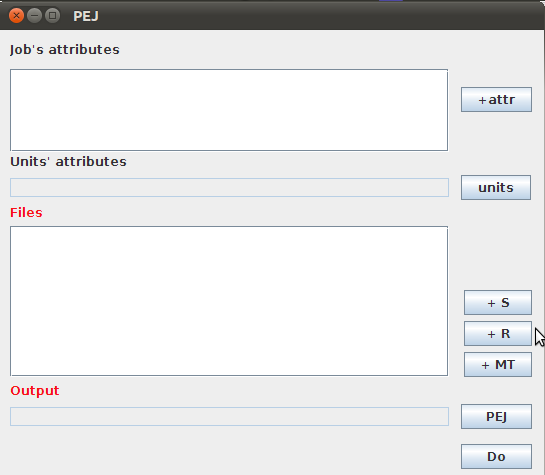
\includegraphics[width=0.5\textwidth]{img/PEJ}
\caption{\PEJ - Auxiliary tool for generating {\tt .pej} files}
\end{figure}


\PEJ (Figure \ref{fig:pejtool}) can format plain text files into {\tt .pej} files for you: run {\tt pej.bat} and a simple interface will be loaded.
\PEJ expects plain text files containing one segment per line. You may input several files for each type of segment (i.e. source, reference, MTs). Each segment must be assigned a producer, therefore the interface will ask either for i) a file-level producer, or ii) a meta file containing attribute-value pairs (one list per line) from where the producer of each segment will be parsed.

\begin{figure}
\centering
\begin{tabular}{|p{3cm} | p{3cm} | p{3cm} | p{3cm} | p{3cm} | }
\hline
\bf \tt Units-attr.txt & \bf \tt S1.txt (opus) & \bf \tt MT1.txt (google) & \bf \tt MT2.txt & \bf \tt MT2-attr.txt\\ \hline \hline
type=pe show=bigbang max=25 & Ela bateu na minha cara. & She slapped me. & She beat me. & producer=model1 \\ \hline
type=pe show=dexter max=20 & Eu nao tenho culpa. & I am not to blame. & Not my fault. & producer=model2 \\ \hline 
\end{tabular}
\caption{\PEJ: example of input files}\label{fig:pejin}
\end{figure}

Figure \ref{fig:pejin} exemplifies input files for \PEJ. These settings will generate a {\tt .pej} file containing two units each one having one source and two machine translations.
The first column is an optional file that may be used to set attributes to each unit. If present this file must specify the attribute {\tt type} of every unit.
The second column is an example of source file, `opus' is the producer of the file, \PEJ will query you for that information.
The third column is an example of machine-translated file, `google' would be the producer.
The fourth column is another example of machine-translated file and the fifth column is an example of a meta file containing attributes for the segments in {\tt MT2.txt}. If present this file must set the producer of every segment.

Figure \ref{fig:pejset} shows an examples of use of \PEJ{}.


\begin{figure}[h]\label{fig:pejset}
\centering
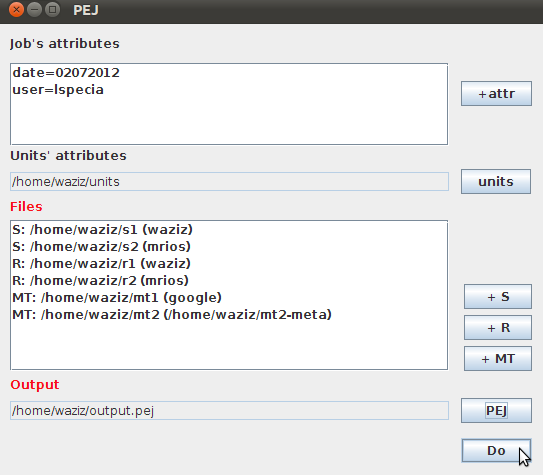
\includegraphics[width=0.5\textwidth]{img/PEJ-settings}
\caption{\PEJ - settings}
\end{figure}

\section{PER}

\PET's output file ({\tt .per}) is a {\tt .pej} file extended with more information - see the example in Listing \ref{lst:per}.
In a {\tt .per} file, the job is tagged with its status and progress, units are also annotated with their status and if a unit has been completed, it will contain a collection of annotations.

\begin{workflow-code}{\PET's output file}{lst:per}
<job id="bigbang-pe-2" progress="1/10" status="GOING_ON">
	<task id="1" status="FINISHED" type="pe">
	<S producer="en-opus">My brother-- he's got a big crush on Bernadette.</S>
	<R producer="pt-opus">Meu irmao... esta apaixonado por Bernadette.</R>
	<MT producer="baseline">meu irmao tem uma quedinha por Bernadette .</MT>
	<MT producer="google">Meu irmao - ele tem uma grande paixao por Bernadette.</MT>
	<MT producer="bing">Meu irmao - ele tem uma grande paixao por Bernadette.</MT>
	<annotations revisions="2">
		<annotation r="1">
			<PE producer="demo.baseline">Meu irmao tem uma quedinha pela Bernadette.</PE>
			<!-- effort indicators ... -->
		</annotation>
		<annotation r="2">
			<PE producer="demo.baseline">Meu irmao tem uma quedinha pela Bernadete.</PE>
			<!-- effort indicators ... -->
		</annotation>
	</annotations>
	</task>
	<!-- ... -->
</job>
\end{workflow-code}

Each revision for each unit contains: i) the human translation (HT) or post-edited text (PE) according to the type of task, with the information on the user who performed the task (e.g. ``demo'' in Listing \ref{lst:per}) and the translation chosen to be edited (e.g. ``baseline'') and depending on the options set in the context file: ii) implicit effort indicators, iii) explicit assessments, and iv) comments.

Listing \ref{lst:indicators} shows the output with explict and implicit effort indicators. Note the timestamped primitive edits (i.e. insertion and deletion) sorted by time and wrapped into more meaningful operations (e.g substitution and shift) when possible.

\begin{workflow-code}{\PET's output file}{lst:indicators}
<job id="bigbang-pe-2" progress="1/10" status="GOING_ON">
  <task id="1" status="FINISHED" type="pe">
    <S producer="en-opus">My brother-- he's got a big crush on Bernadette.</S>
    <R producer="pt-opus">Meu irmao... esta apaixonado por Bernadette.</R>
    <MT producer="baseline">meu irmao tem uma crush por Bernadette .</MT>
    <MT producer="google">Meu irmao - ele tem por Bernadette uma grande paixao.</MT>
    <MT producer="bing">Meu irmao - ele tem uma grande paixao por Bernadette.</MT>
    <annotations revisions="1">
      <annotation r="1">
        <!-- output -->
        <PE producer="demo.baseline">Meu irmao tem uma quedinha por Bernadette.</PE>
        <!-- explicit indicators -->
        <assessment id="adequacy">
          <score>2. Preserves the core</score>
        </assessment>
        <assessment id="fluency">
          <score>2. Minor agreement problems</score>
        </assessment>
        <assessment id="problems">
          <score>Phrase salad</score>
        </assessment>
        <!-- implicit indicators -->
        <indicator id="editing" type="time">50s,2</indicator>
        <indicator id="assessing" type="time">41s,2</indicator>
        <indicator id="keystrokes" type="count">38</indicator>
        <indicator id="white-keystyped" type="count">0</indicator>
        <indicator id="nonwhite-keystyped" type="count">8</indicator>
        <indicator id="iso-keystyped" type="count">8</indicator>
        <indicator id="unchanged" type="flag">false</indicator>
        <!-- timestamped edits -->
        <!-- baseline is shown -->
        <indicator id="target" t0="0,70" type="sysselection">baseline</indicator>
        <indicator elapsed=",0" id="assignment" length="40" offset="0" t0=",71" type="change">meu irmao tem uma crush por Bernadette .</indicator>
        <!-- baseline is replaced by google -->
        <indicator id="target" t0="7s,374" type="sysselection">google</indicator>
        <indicator id="substitution" type="wrap">
          <action elapsed=",0" id="deletion" length="40" offset="0" t0="7s,375" type="change">meu irmao tem uma crush por Bernadette .</action>
          <action elapsed=",0" id="insertion" length="53" offset="0" t0="7s,375" type="change">Meu irmao - ele tem por Bernadette uma grande paixao.</action>
        </indicator>
        <indicator elapsed="2s,260" id="deletion" length="6" offset="10" t0="15s,617" type="change">- ele </indicator>
        <indicator id="shift" type="wrap">
          <action elapsed=",0" id="insertion" length="15" offset="47" t0="29s,623" type="change"> por Bernadette</action>
          <action elapsed="1s,183" id="deletion" length="15" offset="14" t0="34s,157" type="change">por Bernadette </action>
        </indicator>
        <indicator id="substitution" type="wrap">
          <action elapsed=",0" id="deletion" length="14" offset="18" t0="44s,398" type="change">grande paixo.</action>
          <action elapsed="1s,563" id="insertion" length="8" offset="18" t0="44s,399" type="change">quedinha</action>
        </indicator>
        <indicator elapsed=",0" id="insertion" length="1" offset="41" t0="48s,848" type="change">.</indicator>
      </annotation>
    </annotations>
  </task>
\end{workflow-code}

\section{External Information}\label{sec:external}

%\fixme{eu fiquei confusa se vc estava falando de informacao que eh mostrada na bottom pane ou de dicionarios que so mostram informacao quando uma palavra eh right-clicked - please mude o texto abaixo pra deixar isso claro}

XML files are used to bring external information to \PET{}.
External information can be displayed using the bottom boxes shown in Figure \ref{fig:annotation} (referred to as {\it passive info}) or using the drop-down menus shown in Figure \ref{fig:dictionary} (referred to as {\it active info}).
%Dictionaries are examples of files following the conventions discussed in \ref{sec:additional}. 
Either way, the principle is fairly simple, a database of external information is a collections of key-value pairs. 

For {\it passive info} keys are n-grams in the active unit and values are HTML content that will be offered as extra information at the bottom pane. \PET will list in the bottom pane all the information matching n-grams (following the scpecs in the configuration file) of the active unit text at the beginning of the editing.
For {\it active info} keys are n-grams selected by the user and queried via the drop-down menu (for while \PET only renders dictionaries in this way).

\PET does not handle fuzzy matches yet, so the keys are strings to be matched exactly, furthermore the matching of keys is case insensitive.

Listing \ref{lst:pdb-active} shows an example typical of a monolingual dictionary. Values are actively queried by the users when using the drop-down menu.

\begin{workflow-code}{\PET's database file - active}{lst:pdb-active}
<db alias="cambridge">
  <entry>
    <phrase>moving</phrase>
    <paraphrase score="0.36873065">changing place</paraphrase>
  </entry>
  <entry>
    <phrase>moving back</phrase>
    <paraphrase score="0.36873065">going back</paraphrase>
    <paraphrase score="0.36873065">returning</paraphrase>
  </entry>
  <entry>
    <phrase>looks like</phrase>
    <paraphrase score="0.5">appears</paraphrase>
    <paraphrase score="0.2">seems</paraphrase>
  </entry>
</db>
\end{workflow-code}

The entries in Listing \ref{lst:pdb-passive} are definitions and links to external resources (e.g. wikipedia) that are retrieved by \PET when ones starts the editing of a unit.

\begin{workflow-code}{\PET's database file - passive}{lst:pdb-passive}
<db alias="cambridge">
  <entry>
    <phrase>Cholera</phrase>
    <paraphrase>infection in the small intestine caused by the bacterium Vibrio cholerae</paraphrase>
    <paraphrase><a href="http://en.wikipedia.org/wiki/Cholera">wikipedia</a></paraphrase>
  </entry>
  <entry>
    <phrase>Leprosy</phrase>
    <paraphrase>Hansen's disease</paraphrase>
    <paraphrase><a href="http://en.wikipedia.org/wiki/Leprosy">wikipedia</a></paraphrase>
  </entry>
  <entry>
    <phrase>Hansen's disease</phrase>
    <paraphrase>leprosy</paraphrase>
    <paraphrase><a href="http://en.wikipedia.org/wiki/Leprosy">wikipedia</a></paraphrase>
  </entry>  
</db>
\end{workflow-code}

In Listings \ref{lst:pdb-active} and \ref{lst:pdb-passive} an entry has a key `phrase' and a list of values each one identified by the tag `paraphrase'. A score may be also given. For example, if multiple paraphrases are available, a score reflecting their length could be of use in experiments where the length of the translation is important. Frequency or confidence scores can also be useful.	

